
\newcommand{\matrixe}[3]{\ensuremath{\langle{#1}|\,{#2}\,|{#3}\rangle}}
\newcommand{\rmatrixe}[3]{\ensuremath{ \abrapar {#1} \big|\big| \,{#2}\, \big|\big| {#3} \aketpar }}


\newcommand{\comm}[2]{\ensuremath{[{#1},{#2}]}}
\newcommand{\acomm}[2]{\ensuremath{ \big\{ {#1}, {#2} \big\} }}

\newcommand{\op}[1]{\ensuremath{#1}}
\newcommand{\adj}[1]{\ensuremath{{{#1}}^{\dag}}}

\renewcommand{\vec}[1]{\ensuremath{\bm{#1}}}


\newcommand{\totd}[2]{\ensuremath{ \frac{d {#1}} {d {#2}} }}

%%%%% normal ordering
\newcommand{\nord}[1]{\ensuremath{\,:\!#1\!:\,}}

%%%%% operator shortcuts
\newcommand{\aO}{\ensuremath{\hat{a}}}
\newcommand{\hO}{\ensuremath{\hat{h}}}
\newcommand{\etaO}{\ensuremath{\hat{\eta}}}

\newcommand{\aaO}{\ensuremath{\adj{\hat{a}}}}
\newcommand{\ccO}{\ensuremath{\adj{\hat{c}}}}
\newcommand{\UUO}{\ensuremath{\adj{\hat{U}}}}
\newcommand{\Deltaz}{\ensuremath{\overline{\Delta}^{[0]}}}
\newcommand{\Deltat}{\ensuremath{\overline{\Delta}^{[2]}}}
\newcommand{\etao}{\ensuremath{\overline{\eta}^{[1]}}}
\newcommand{\etat}{\ensuremath{\overline{\eta}^{[2]}}}
\newcommand{\etath}{\ensuremath{\overline{\eta}^{[2]}}}
\newcommand{\Gammao}{\ensuremath{\overline{\Gamma}^{[1]}}}
\newcommand{\Gammat}{\ensuremath{\overline{\Gamma}^{[2]}}}
\newcommand{\Gammath}{\ensuremath{\overline{\Gamma}^{[3]}}}
\newcommand{\Wt}{\ensuremath{\overline{W}^{[2]}}}
\newcommand{\diag}{\operatorname{diag}}


\title{In-medium SRG approaches to infinite nuclear matter}
\author{Scott K.~Bogner, Heiko Hergert, Justin Leitz, Titus Morris, Sam Novario, Nathan Parzuchowski, and Fei Yuan}
\institute{Scott Bogner  \at Department of Physics and Astronomy and National Superconducting Cyclotron Laboratory, Michigan State University, East Lansing, Michigan USA, \email{bogner@nscl.msu.edu}, \and Heiko Hergert  \at Department of Physics and Astronomy and National Superconducting Cyclotron Laboratory, Michigan State University, East Lansing, Michigan USA, \email{hergert@nscl.msu.edu}, \and Justin G.~Lietz \at Department of Physics and Astronomy and National Superconducting Cyclotron Laboratory, Michigan State University, East Lansing, Michigan,  USA, \email{lietz@nscl.msu.edu}, \and Titus Morris  \at Department of Physics and Astronomy and National Superconducting Cyclotron Laboratory, Michigan State University, East Lansing, Michigan USA, \email{morrist@nscl.msu.edu}, \and Samuel Novario \at Department of Physics and Astronomy and National Superconducting Cyclotron Laboratory, Michigan State University, East Lansing, Michigan,  USA, \email{novarios@nscl.msu.edu},\and Nathan Parzuchowski  \at Department of Physics and Astronomy and National Superconducting Cyclotron Laboratory, Michigan State University, East Lansing, Michigan USA, \email{parzuchowski@frib.msu.edu}, \and Fei Yuan  \at Department of Physics and Astronomy and National Superconducting Cyclotron Laboratory, Michigan State University, East Lansing, Michigan USA, \email{yuan@nscl.msu.edu}}
\maketitle
\abstract{We present applications  of the In-Medium Similarity
Renormalization Group (IM-SRG) method to studies of infinite nuclear matter. 
The IM-SRG method employs a continuous unitary transformation of the
many-body Hamiltonian to decouple the ground state from all
excitations, thereby solving the many-body problem. Starting from a
pedagogical introduction of the underlying concepts, the IM-SRG flow 
equations are developed and we study different IM-SRG generators that
achieve the desired decoupling, and how they affect the details of the IM-SRG results. We compare with the coupled cluster theory results of
chapter 8, the Monte Carlo results of chapter 9 and the Green's function results of chapter 11.}

\section{Introduction}

The Similarity Renormalization Group (SRG) method was first formulated by
Wegner \cite{wegner1994} and Glazek and Wilson \cite{glazek1993}
to study condensed matter systems and light-front quantum field
theories, respectively.  From a mathematical point of view, the
philosophy behind the SRG is to render the Hamiltonian $\hat{H}(s)$
diagonal via a continuous unitary transformation
\begin{equation}\label{eq:cut}
  \hat{H}(s)=\hat{U}(s)\hat{H}(0)\UUO(s)\,,
\end{equation}
where $H(s=0)$ is the starting Hamiltonian and $s$ denotes the so-called flow
parameter, for reasons that will become apparent shortly. In practice, the demand 
for strict diagonality is usually relaxed to requiring band- or block-diagonality 
of the Hamiltonian matrix in a chosen basis
These specific cases are realized in nuclear
physics applications, where the SRG is used to decouple momentum or
energy scales, and thereby render the nuclear Hamiltonian more
suitable for \emph{ab initio} many-body calculations \cite{bogner2007,bogner2010,morris2015,bogner2016}.

In the following sections we outline the basic ingredients behind the
SRG method, with an emphasis on applications to infinite nuclear
matter, coupling our final results with those of chapter 8, 9 and
11. The next section presents the essential philosophy of the method,
which in practice means to solve Schr\"odinger's equation for a
many-body system in terms of coupled ordinary differential equations
(ODEs). We present also two simple demonstrations of the method before
presenting our applications to infinite neutron matter with a
cartesian basis. In the final section, we point to further
perspectives.

\section{Similarity Renormalization Group method}

We give here a brief overview of the SRG method applied to two simple systems, one given by a $2\times 2$ matrix and its pertinent eigenvalue problem and the simple pairing model discussed in chapter 8. 

Taking the derivative of Eq.~\eqref{eq:cut}
with respect to the flow parameter $s$, we obtain the operator flow equation
\begin{equation}\label{eq:opflow}
  \totd{}{s}\hat{H}(s) = \comm{\etaO(s)}{\hat{H}(s)},
\end{equation} 
where the generator $\etaO(s)$ is related to the unitary transformation $\hat{U}(s)$ by
\begin{equation}
  \eta(s)=\totd{U(s)}{s}U^{\dag}(s) = -\eta^{\dag}(s).
\end{equation}
By rearranging this relation, we obtain a differential equation for $\hat{U}(s)$ whose formal solution is given by the \emph{path-}
or \emph{S-ordered} exponential
\begin{equation}
  U(s) = \mathcal{S}\exp \int^s_0 ds' \eta(s').
\end{equation}
We leave $\etaO(s)$ unspecified for now and defer the discussion of suitable choices to section \ref{sec:generators}. 

Naively, one could try to solve the flow equation \eqref{eq:opflow} by
choosing a suitable basis of the many-body Hilbert space and turning
Eq.~\eqref{eq:opflow} into a matrix differential equation, but such an
approach would ultimately amount to a diagonalization of the many-body
Hamiltonian. To make matters worse, implementing the flow means we
would deal with the Hamiltonian's full spectrum rather than just some
extremal eigenvalues that can be extracted efficiently in
state-of-the-art, large-scale Lanczos approaches like the 
\cite{navratil2000,barrett2013}.

\subsection{Simple demonstration of the SRG method}
Let us study a simple $2\times 2$ matrix and use Jacobi's rotation method \cite{golubvanloan1996} to find its eigenvalues. 
We will thereafter link the flow equations
with the results obtained with the simple Jacobi method, see for example Ref.~\cite{golubvanloan1996}.

We define a  symmetric matrix  $H\in {\mathbb{R}}^{2\times 2}$
\[ 
H = \begin{bmatrix} H_{11} & H_{12} \\ H_{21} & H_{22}\end{bmatrix}. 
\]
The standard Jacobi rotation method allows us to find the eigenvalues via the orthogonal matrix
$\mathbf{U}$ 
\[ 
\mathbf{U} = \begin{bmatrix} c & s \\ -s & c
\end{bmatrix}, 
\]
with $c = \cos \gamma$ and $s = \sin \gamma$. We have then that  $H' = UHU^T$ is diagonal. 

To have non-zero nondiagonal matrix $H'$ we need to solve
\[ 
(H_{22} - H_{11})cs + H_{12}(c^2 - s^2) = 0, 
\]
and using $c^2-s^2 = \cos(2\gamma)$ and $cs = \sin(2\gamma)/2$
this is equivalent with 
\[ \tan(2\gamma) = \frac{2 H_{12}}{H_{11}-H_{22}}. \]
Solving the equation we have
\begin{equation} 
\gamma = \frac{1}{2} \tan^{-1} \left( \frac{2H_{12}}{H_{11}-H_{22}}
\right) + \frac{k\pi}{2}, \quad k=\ldots,-1,0,1,\ldots, \label{eq:0} 
\end{equation}
where $k\pi/2$ is added due to the periodicity of the $\tan$ function.

Note that  $k=0$ gives a diagonal matrix on the form
\begin{equation} 
H'_{k=0} = \begin{bmatrix} \lambda_1 & 0 \\ 0 & \lambda_2 \end{bmatrix},
\label{eq:1} 
\end{equation}
while  $k=1$ changes the diagonal elements  
\begin{equation} 
H'_{k=1} = \begin{bmatrix} \lambda_2 & 0 \\ 0 & \lambda_1 \end{bmatrix}.
\label{eq:2}
\end{equation}

We switch now to the SRG method and 
let $H(s) = T + V(s)$, where $T= \diag(E_1,E_2)$ is diagonal. We want to solve the ordinary differential equations (ODEs) 
for $U(s)$ using the flow parameter $s$. 
We have not
\[ 
H(s) = U(s)H(0)U(s)^T, 
\]
and we have
\[ 
\frac{d}{ds} H(s) = [\eta(s),H(s)],  \quad \eta(s) = [T,H(s)], 
\]
which gives
\[ 
\frac{d}{ds} U(s) = \eta(s) U(s). 
\]
Note that $\eta(s)^T = -\eta(s)$, that is
\[ 
\eta(s) = \begin{bmatrix} 0 & a(s) \\ -a(s) & 0 \end{bmatrix}. 
\]

To make the link with the Jacobi rotation
we can parameterize $U(s)$ as
\[ 
U = \begin{bmatrix} \cos(\gamma(s)) & \sin(\gamma(s)) \\ -\sin(\gamma(s)) & \cos(\gamma(s)) \end{bmatrix}. 
\]
Setting up $\eta(s)U(s)$ og $\frac{d}{ds} U(s)$ we arrive at 
\[ 
\frac{d}{ds} \gamma(s) = a(s). 
\]

We rewrite $H(s)$ (and $T$ and $V(s)$)  via Pauli matrices
\[ 
T = \mathcal{E} I + \Omega \sigma_z, \quad \mathcal{E} = \frac{E_1
  + E_2}{2}, \; \Omega = \frac{E_1-E_2}{2}, 
\]
and
\[ 
V(s) = c I \omega_z(s)\sigma_z + \omega_x(s)\sigma_x, 
\]
with $c = (V_{11}+V_{22})/2$, $\omega_z(s) = (V_{11}-V_{22})/2$,
$\omega_x(s) = V_12$. The quantities depend on
$s$. 

We obtain
\[ \eta(s) = [T, H(s)] = 2\Omega\omega_x(s)\sigma_y, \]
where we have used $\sigma_i\sigma_j = i\epsilon_{ijk}\sigma_k$.
It results in
\[ a(s) = 2\Omega \omega_x(s), \]
and $\gamma(s)$,
\begin{equation} \frac{d}{ds} \gamma(s) = 2\Omega\omega_x(s). \label{eq:3}\end{equation}

We introduce next the  variables $\omega(s)$ and $\theta(s)$ instead of
$\omega_x(s)$ and $\omega_y(s)$. 

We obtain an ODE for $\theta(s)$ 
\begin{equation} 
\frac{d}{ds} \theta(s) = -4\Omega\omega \sin(\theta(s)), \label{eq:4}
\end{equation}
and noting that
\[ 
\frac{d}{dx} \ln \tan \frac{x}{2} = \frac{1}{\sin x}, 
\]
we get
\[ 
\tan\left(\frac{\theta(s)}{2}\right) = \exp{-4\Omega\omega s} \tan\left(
  \frac{\theta(0)}{2}\right). 
\]
If $\Omega<0$ ($E_1-E_2<0$) we obtain  $\theta(s)\rightarrow \pi$, and if 
$\Omega>0$ we get  $\theta(s)\rightarrow 0$. 

Exponential convergence. In a compact form
\begin{equation} \theta(s) \rightarrow \pi \vartheta(E_2 - E_1),
  \label{eq:5} \end{equation}
where $\vartheta(x)$ is the  step function.

Recall also that 
\[ \tan \theta(0) = \frac{2 V_{12}(0) }{[E_1 + V_{11}(0)]- [E_2 +
  V_{22}(0)]},
\]
to be linked with the Jacobi  rotation.

Now comes the point: comparing the  ODE of (\ref{eq:3}) with 
(\ref{eq:4}), we have
\[ \frac{d}{ds} \gamma(s) = -\frac{1}{2} \frac{d}{ds} \theta(s). \]
The initial condition is 
$\gamma(0) = 0$. Integrating we have
\[ \gamma(s) = \frac{1}{2}\theta(0) - \frac{1}{2}\theta(s). \]
Using (\ref{eq:5}) results in 
\[ \gamma(s) \rightarrow \frac{1}{2}\theta(0) -
\frac{\pi}{2}\vartheta(E_2-E_1). \]

From this we see that the flow equation selects the solution of (\ref{eq:0}) with
$k=0$ and $k=-1$, depending on whether  $E_1<E_2$ or
$E_2<E_1$.

The flow equation yields $H(s)$ as a continuous function of $s$ and the solution
$H(\infty)$ results in the eigenvalues sorted the same way as
$T = \diag(E_1,E_2)$. The shift $\pi/2$ is connected with this; if $k=0$ in 
(\ref{eq:0}) gives the wrong sequence, we choose $k=-1$ instead!

\subsection{The pairing model}

\section{In-medium SRG and flow equations}

For the IM-SRG, we follow a different route, and formulate the flow equation as well as the decoupling conditions underlying the definition of $\etaO(s)$ in the language of second quantization. This approach has been very successful in producing powerful and numerically efficient many-body schemes, chief among them the coupled cluster method discussed in chapter 8.

When carried out exactly, the IM-SRG is a continuous unitary transformation in $A$-body space, and consequently, $\eta(s)$ and $\hat{H}(s)$ are $A$-body operators even if they initially have a lower rank at $s=0$. From the discussion of the previous sections, we see that every evaluation of the commutator on the right-hand side of Eq.~\eqref{eq:opflow} increases the particle rank of $\hat{H}(s)$, e.g.,
\begin{equation}\label{eq:induced}
  \comm{\nord{\aaO_{a}\aaO_{b}\aO_{d}\aO_{c}}}{\nord{\aaO_{i}\aaO_{j}\aO_{l}\aO_{k}}}= \delta_{ci}\nord{\aaO_{a}\aaO_{b}\aaO_{j}\aO_{l}\aO_{k}\aO_{d}}+\ldots.
\end{equation}
All of these induced contributions will in turn contribute to the
parts of $\hat{H}(s)$ with lower particle rank in subsequent integration
steps. Because an explicit treatment of all contributions up to the
$A$-body level is clearly not feasible, we have to introduce a
truncation to close the system of IM-SRG flow equations. We follow a
simple approach, and truncate $\etaO(s)$ and $\hat{H}(s)$ at a given
particle rank $n\leq A$, which is motivated by the cluster
decomposition principle for short-range interactions (see, e.g.,
\cite{weinberg1996}). For $n=2$, this yields the so-called
IM-SRG(2) truncation, our primary truncation scheme in past works
\cite{tsukiyama2011,tsukiyama2012,hergert2013}, which will
serve as the basis of the discussion in the remainder of this work. 

Let us assume, then, that for each flow parameter $s$
\begin{align}
  \hat{H}(s) &\approx E(s) + f(s) + \Gamma(s)\,,\\
  \etaO(s) &\approx\etaO^{(1)}(s)+\etaO^{(2)}(s)\,.
\end{align}
We introduce the permutation symbol $P_{ij}$ to interchange the attached indices in any expression, i.e.,
\begin{equation}\label{eq:def_Pij}
  P_{ij} g(\ldots,i,\ldots,j) \equiv g(\ldots,j,\ldots,i)\,,
\end{equation}
and use the fundamental commutators from Appendix \ref{app:commutators} to obtain
\begin{align}
  \totd{E}{s}&= \sum_{ab}(n_a-n_b)\eta_{ab} f_{ba} 
    + \frac{1}{2} \sum_{abcd}\eta_{abcd}\Gamma_{cdab} n_a n_b\bar{n}_c\bar{n}_d
    \label{eq:imsrg2_m0b}\,,\\[5pt]
% \end{align}
% 
% \begin{align}
  \totd{f_{12}}{s} &= 
  \sum_{a}(1+P_{12})\eta_{1a}f_{a2} +\sum_{ab}(n_a-n_b)(\eta_{ab}\Gamma_{b1a2}-f_{ab}\eta_{b1a2}) \notag\\ 
  &\quad +\frac{1}{2}\sum_{abc}(n_an_b\bar{n}_c+\bar{n}_a\bar{n}_bn_c) (1+P_{12})\eta_{c1ab}\Gamma_{abc2}
  \label{eq:imsrg2_m1b}\,,\\[5pt]
% \end{align}
% 
% \begin{align}
  \totd{\Gamma_{1234}}{s}&= 
  \sum_{a}\left\{ 
    (1-P_{12})(\eta_{1a}\Gamma_{a234}-f_{1a}\eta_{a234} )
    -(1-P_{34})(\eta_{a3}\Gamma_{12a4}-f_{a3}\eta_{12a4} )
    \right\}\notag \\
  &\quad+ \frac{1}{2}\sum_{ab}(1-n_a-n_b)(\eta_{12ab}\Gamma_{ab34}-\Gamma_{12ab}\eta_{ab34})
    \notag\\
  &\quad-\sum_{ab}(n_a-n_b) (1-P_{12})(1-P_{34})\eta_{b2a4}\Gamma_{a1b3}
    \label{eq:imsrg2_m2b}\,,
\end{align}
% \end{widetext}
where $\bar{n}_i=1-n_i$, and the $s$-dependence has been suppressed for brevity. To obtain ground-state energies, we integrate Eqs.~\eqref{eq:imsrg2_m0b}--\eqref{eq:imsrg2_m2b} from $s=0$ to $s\to\infty$, starting from the initial 
components of the normal-ordered Hamiltonian (Eqs.~\eqref{eq:E0}--\eqref{eq:Gamma}).

As we will discuss in more detail in Sec.~\ref{sec:mbpt}, 
Eqs.~\eqref{eq:imsrg2_m0b}--\eqref{eq:imsrg2_m2b} can easily be translated 
into Goldstone or Hugenholtz diagrams for the flowing Hamiltonian $H(s)$.
This provides us with an intuitive understanding of the mechanism through
which the IM-SRG is non-perturbatively re-summing the many-body expansion. The second
and third rows of Eq.~\eqref{eq:imsrg2_m2b}, in particular, re-sum $pp/hh$-ladder and $ph$-ring 
diagrams, respectively. Due to the use of $H(s)$, ladder-ring interference 
diagrams are generated in the limit $s\to\infty$, and therefore the IM-SRG(2) 
goes beyond the more traditional Brueckner $G$-matrix or Random-Phase 
Approximation-type summations \cite{Day:1967zl,Brandow:1967tg,Fetter:2003ve}. 
Furthermore, the commutator structure of Eq.~\eqref{eq:opflow} ensures that 
the IM-SRG is size-extensive, and only connected diagrams are generated and
re-summed by the IM-SRG flow \cite{Brandow:1967tg,Shavitt:2009}. This property
is preserved even if the commutators are truncated at a given operator rank, as in the IM-SRG(2) case presented here. 

From Eqs.~\eqref{eq:imsrg2_m0b}--\eqref{eq:imsrg2_m2b}, it is clear
that the computational effort for solving the IM-SRG(2) flow equations
is dominated by the two-body flow equation, which scales polynomially
like $\mathcal{O}(N^6)$ with the single-particle basis size $N$. This puts the
IM-SRG(2) in the same category as other numerically efficient
non-perturbative methods\footnote{The mentioned methods can make use
  of the distinction between particle and hole states in the
  single-particle basis to further reduce the effort. For instance,
  the amplitude equations of CCSD can be solved at $\mathcal{O}(N_h^2N_p^4)$
  cost, where typically the number of hole states $N_h$ is much
  smaller than the number of particle states $N_p\sim N$. Note that
  the construction of the CCSD effective Hamiltonian from the
  amplitudes requires $\mathcal{O}(N^6)$ effort. In the IM-SRG(2), we are
  working directly with the analogous effective Hamiltonian.} like
Coupled Cluster with Singles and Doubles (CCSD)
\cite{Shavitt:2009,Hagen:2014ve}, the Self-Consistent Green's Function
Approach (SCGF)
\cite{Dickhoff:2004fk,Barbieri:2007fk,Cipollone:2013uq}, or canonical
transformation theory \cite{White:2002fk,Yanai:2006uq}.

\subsection{General Observables\label{sec:observables}}
In principle, the evaluation of observables other than the Hamiltonian
is a straightforward task: We need to normal-order the operator
$\hat{O}(s)$ with respect to the same reference state as the Hamiltonian,
and then plug it into the flow equation
\begin{equation}\label{eq:obsflow}
  \totd{}{s}\hat{O}(s) = \comm{\etaO(s)}{\hat{O}(s)}\,,
\end{equation} 
with $\etaO(s)$ the same as in the Hamiltonian flow equation. For
consistency with the overall IM-SRG(2) scheme, $\hat{O}(s)$ is truncated
at the two-body level. We then obtain an additional set of flow
equations for the normal-ordered zero-, one- and two-body parts of
$\hat{O}(s)$ which need to be solved alongside
Eqs.~\eqref{eq:imsrg2_m0b}--\eqref{eq:imsrg2_m2b}. We will follow this
route in later sections of this work to investigate radii
(Sec.~\ref{sec:numerics_radii}) and the center-of-mass separation in
the IM-SRG(2) ground-state wave function (Sec.~\ref{sec:com}). Due to
the size of the system of flow equations, and the associated storage
needs of numerical differential equation solvers, this procedure
becomes unfeasible if we are interested in more than one or two
additional operators.

Unfortunately, we cannot resort to the same strategy as in the
free-space SRG case \cite{Anderson:2010br,Bogner:2010pq}, where the
unitary transformation can be reconstructed from the eigenvectors of
the initial and final Hamiltonians in the two-nucleon,
three-nucleon,\ldots system. To do so, we would have to solve the
eigenvalue problem of the Hamiltonian in the $A$-body system through
exact diagonalization, and we could not even resort to large-scale
NCSM machinery because it does not provide the full eigenbasis, but
only the lowest eigenvalues and eigenvectors via Lanczos methods. The
cost for exact diagonalization increases factorially with the
single-particle basis, and it is precisely this high computational
effort that motivated the development of mildly scaling methods like
CC or the IM-SRG. A more efficient alternative for the evaluation of
observables exists in the form of the so-called Magnus expansion
\cite{Blanes:2009fk,Morris:2015ve}, which we briefly discuss in
Sec.~\ref{sec:magnus}.



\section{\label{sec:generators}Choice of Generator}

\subsection{\label{sec:decoupling}Decoupling}
\begin{figure}[t]
\setlength{\unitlength}{0.8\columnwidth}
  \begin{center}
  \begin{picture}(1.0000,0.5500)
   \put(0.0350,0.0450){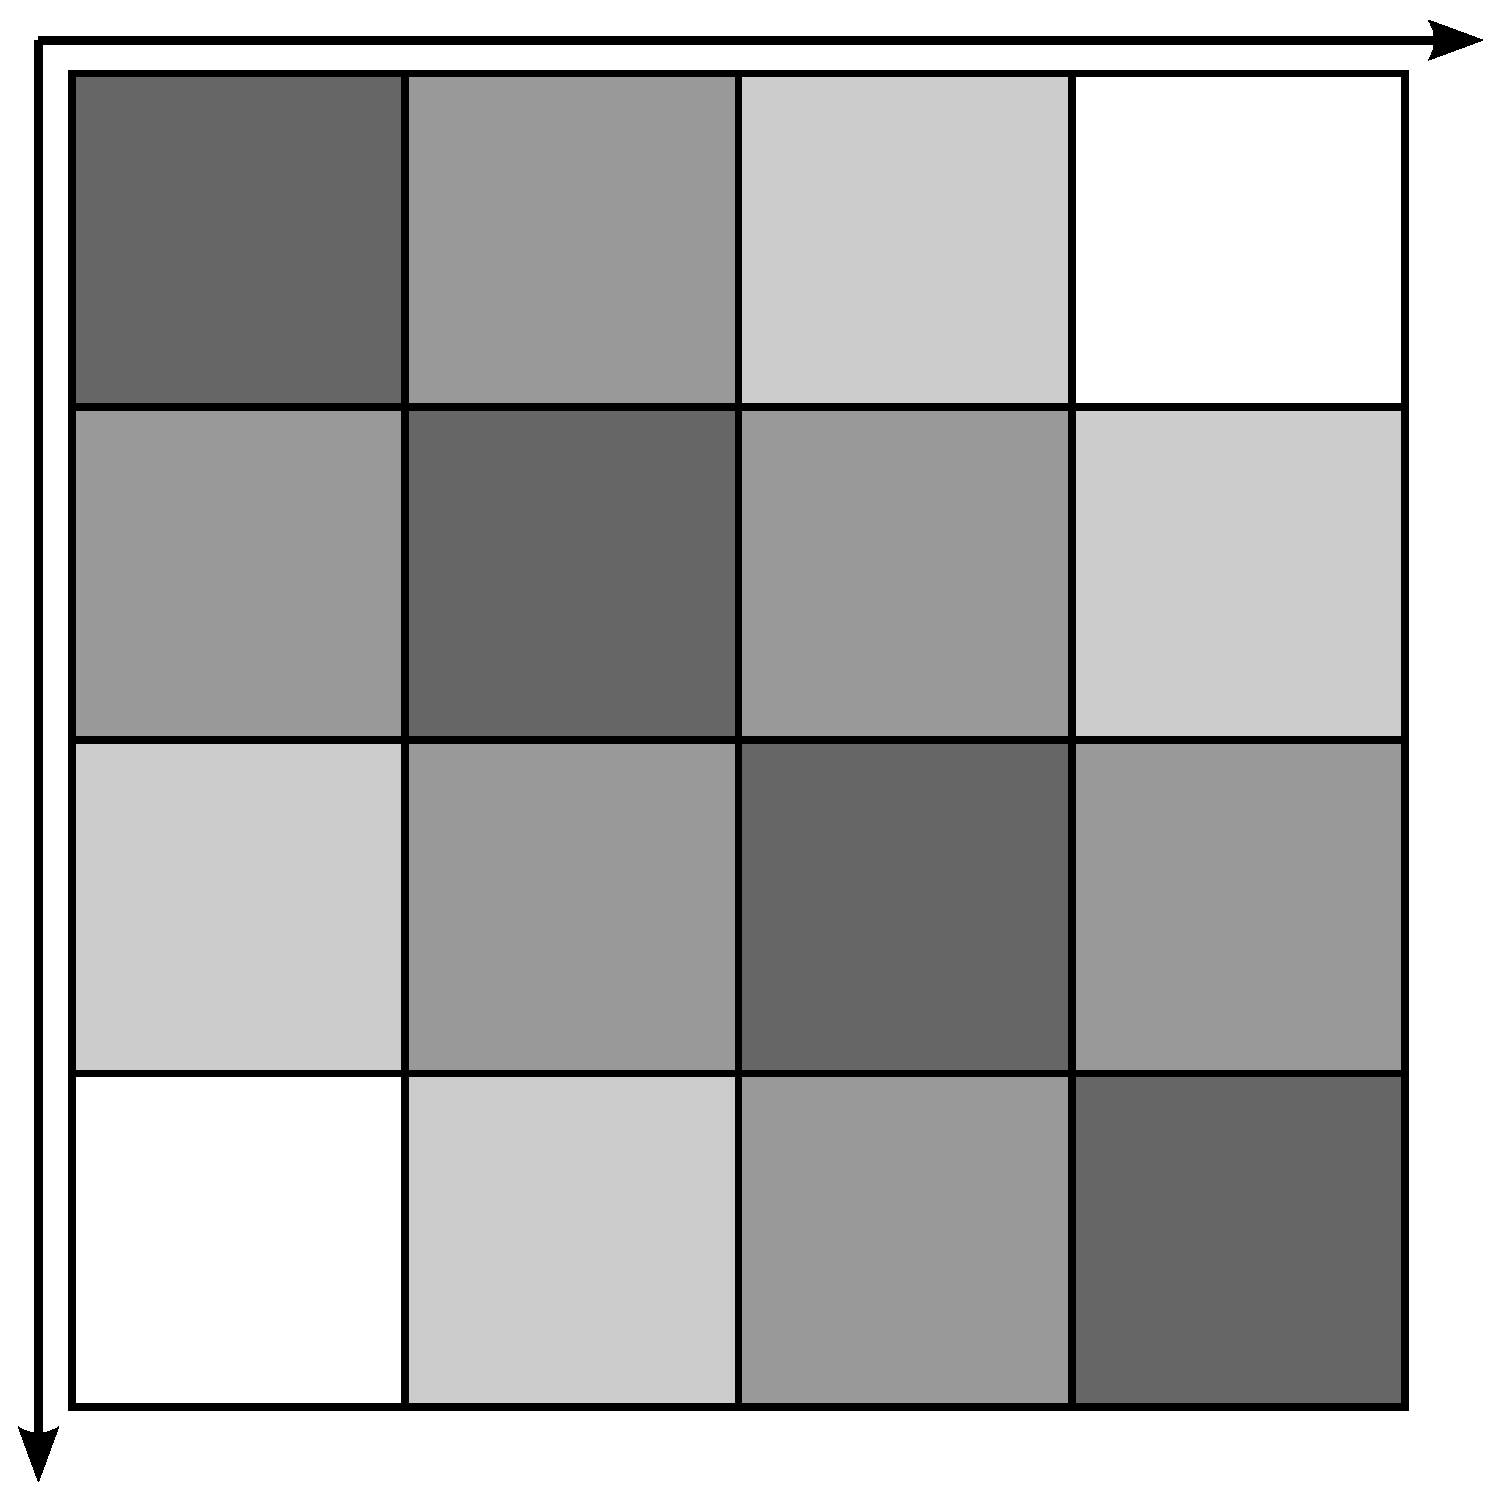
\includegraphics[width=0.46\unitlength]{Chapter10-figures/H_initial.eps}}
   \put(0.5400,0.0450){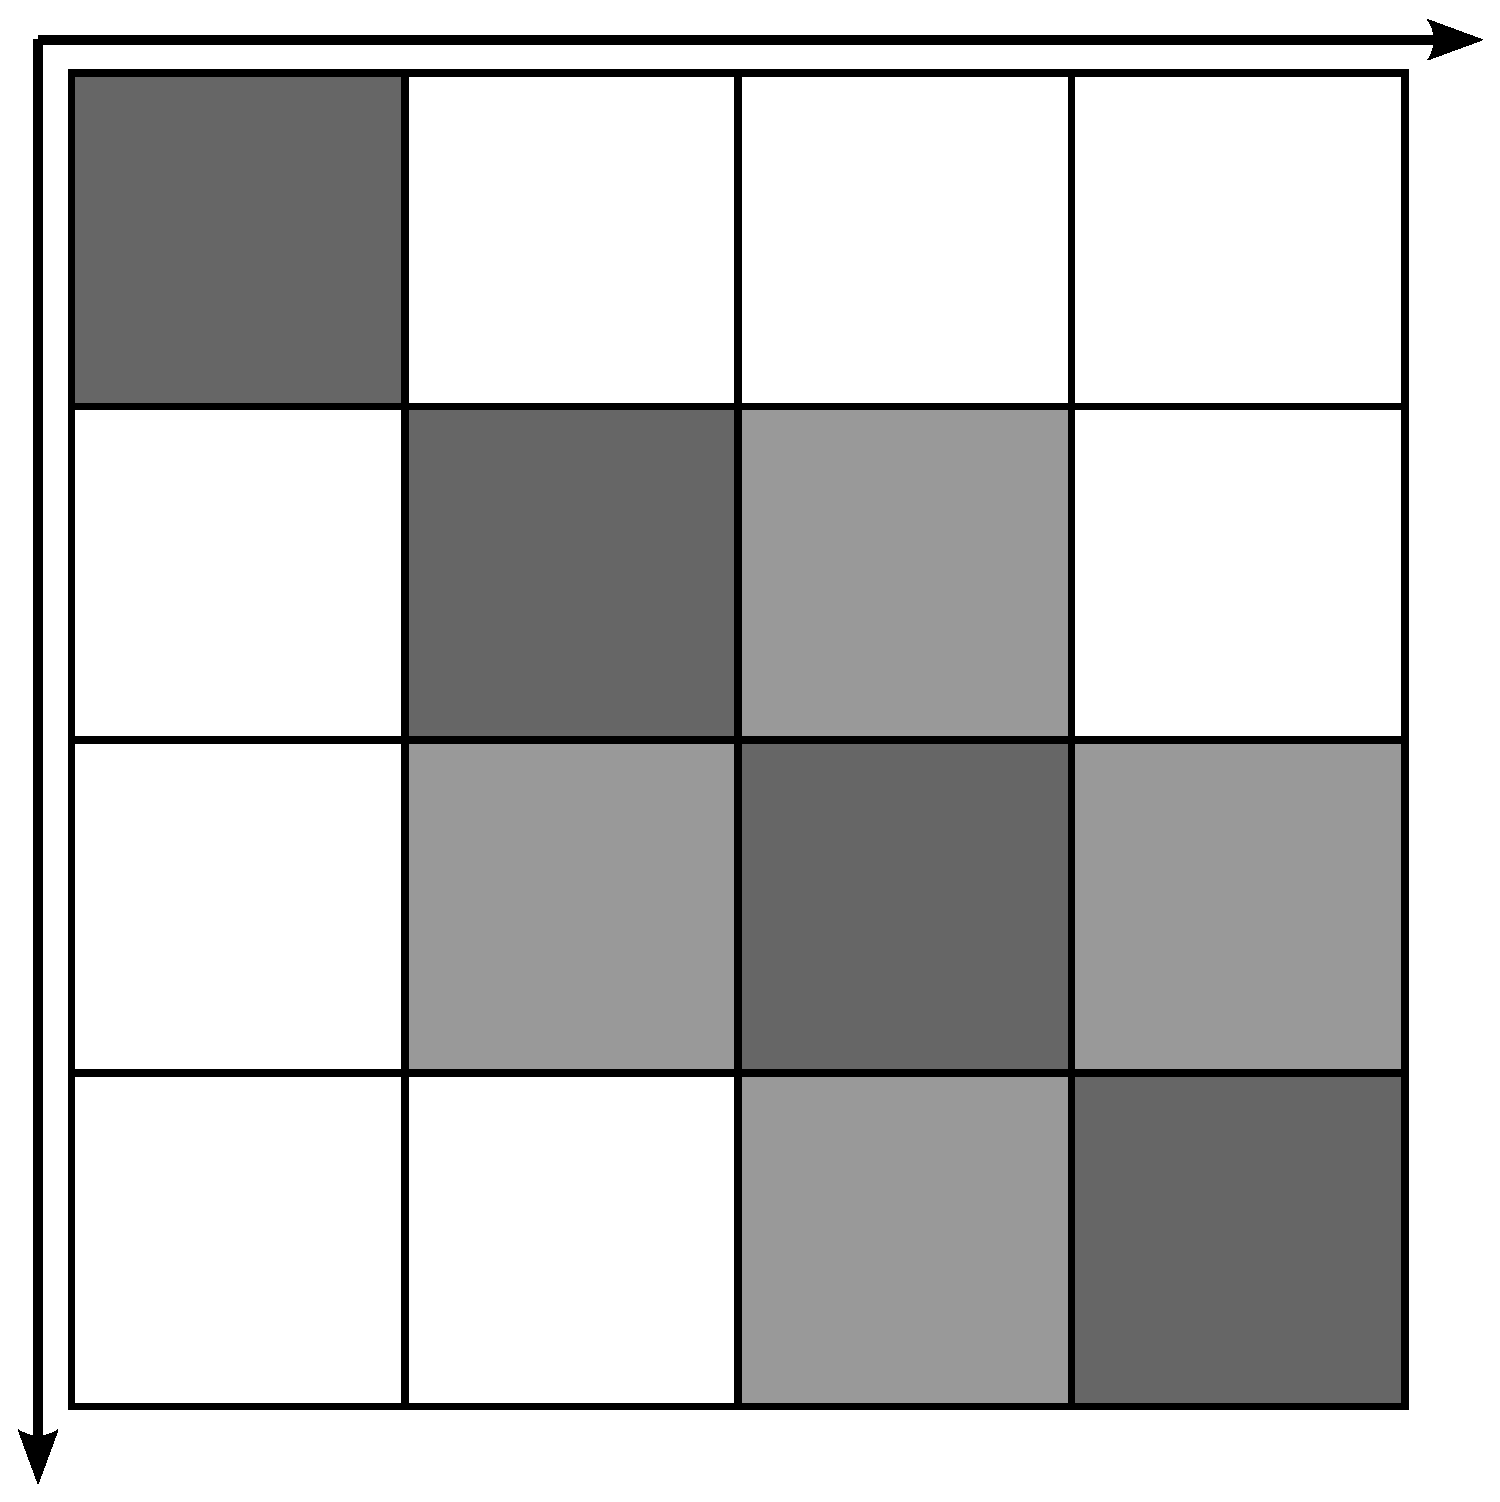
\includegraphics[width=0.46\unitlength]{Chapter10-figures/H_IMSRG_3ph_decoupling.eps}}
   \put(0.0100,0.0000){\parbox{0.5\unitlength}{\centering$\matrixe{i}{\hat{H}(0)}{j}$}}
   \put(0.5200,0.0000){\parbox{0.5\unitlength}{\centering$\matrixe{i}{\hat{H}(\infty)}{j}$}}
   
   \put(0.0500,0.5100){\parbox{0.11\unitlength}{\centering\footnotesize0p0h}}
   \put(0.1600,0.5100){\parbox{0.11\unitlength}{\centering\footnotesize1p1h}}
   \put(0.2630,0.5100){\parbox{0.11\unitlength}{\centering\footnotesize2p2h}}
   \put(0.3650,0.5100){\parbox{0.11\unitlength}{\centering\footnotesize3p3h}}
   \put(0.5500,0.5100){\parbox{0.11\unitlength}{\centering\footnotesize0p0h}}
   \put(0.6600,0.5100){\parbox{0.11\unitlength}{\centering\footnotesize1p1h}}
   \put(0.7630,0.5100){\parbox{0.11\unitlength}{\centering\footnotesize2p2h}}
   \put(0.8650,0.5100){\parbox{0.11\unitlength}{\centering\footnotesize3p3h}}
  %
   \put(0.0100,0.4320){\parbox{0.11\unitlength}{\rotatebox{90}{\centering\footnotesize0p0h}}}
   \put(0.0100,0.3235){\parbox{0.11\unitlength}{\rotatebox{90}{\centering\footnotesize1p1h}}}
   \put(0.0100,0.2175){\parbox{0.11\unitlength}{\rotatebox{90}{\centering\footnotesize2p2h}}}
   \put(0.0100,0.1100){\parbox{0.11\unitlength}{\rotatebox{90}{\centering\footnotesize3p3h}}}

   \put(0.5100,0.4320){\parbox{0.11\unitlength}{\rotatebox{90}{\centering\footnotesize0p0h}}}
   \put(0.5100,0.3235){\parbox{0.11\unitlength}{\rotatebox{90}{\centering\footnotesize1p1h}}}
   \put(0.5100,0.2175){\parbox{0.11\unitlength}{\rotatebox{90}{\centering\footnotesize2p2h}}}
   \put(0.5100,0.1100){\parbox{0.11\unitlength}{\rotatebox{90}{\centering\footnotesize3p3h}}}
  \end{picture}
  \end{center}
  \caption{\label{fig:schematic}Schematic representation of the initial and final Hamiltonians, $\hat{H}(0)$ and $\hat{H}(\infty)$, in the many-body Hilbert space spanned by particle-hole excitations of the reference state.}
\end{figure}

After setting up the general IM-SRG flow equation framework in
Sec.~\ref{sec:floweq}, we have to specify the generator $\etaO$. To
this end, we first need to identify the off-diagonal parts of the
Hamiltonian that the IM-SRG transformation is supposed to suppress for
$s\to\infty$. The freedom to partition the Hamiltonian into suitably
defined diagonal and off-diagonal pieces gives the IM-SRG flexibility
to target different states, and is key to extending the method to
open-shell nuclei, see Secs.~\ref{sec:mrimsrg} and
\ref{sec:shell_model}. To illustrate the general idea of a targeted
decoupling, let us assume our goal is to extract the ground-state
energy of a closed-shell nucleus, i.e., the lowest eigenvalue of the
nuclear many-body Hamiltonian. In the left panel of
Fig.~\ref{fig:schematic}, we show a schematic representation of the
initial Hamiltonian $\hat{H}(0)$, in a basis consisting of
$A$-particle-$A$-hole ($A$p$A$h) excitations of the reference state
$\ket{\Phi}$. For the following illustration of the IM-SRG's basic
concept, we assume that $\hat{H}(0)$ has been truncated to two-body
operators, that is, it can at most couple $n$p$n$h to
$(n\pm2)$p$(n\pm2)$h states. The extension to three-body operators is
straightforward.

The 0p0h reference state is coupled to 1p1h and 2p2h excitations by the matrix elements
\begin{align}
  \matrixe{\Phi}{\hat{H}(0)\nord{\aaO_{p}\aO_{h}}}{\Phi}&=f_{ph}\,,\label{eq:fod}\\
  \matrixe{\Phi}{\hat{H}(0)\nord{\aaO_{p}\aaO_{p'}\aO_{h'}\aO_{h}}}{\Phi}&=\Gamma_{pp'hh'}\label{eq:Gammaod}\,,
\end{align}
and their Hermitian conjugates. Thus, we define the off-diagonal part of the Hamiltonian as
\begin{equation}
  \hat{H}^{od}(s) = \sum_{ph}f_{ph}\nord{\aaO_p\aO_h} + \frac{1}{4}\sum_{pp'hh'}\Gamma_{pp'hh'}\nord{\aaO_p\aaO_{p'}\aO_{h'}\aO_h}
                +\; \text{H.c.}\label{eq:def_Hod}\,.
\end{equation}
During the flow, matrix elements between the reference state and higher excitations acquire non-zero values,
\begin{equation}\label{eq:induced_od}
  \matrixe{\Phi}{\hat{H}(s)\nord{\aaO_{p_1}\ldots\aaO_{p_A}\aO_{h_{A}}\ldots\aO_{h_1}}}{\Phi}\neq 0\,,
\end{equation}
because $\hat{H}(s>0)$ has induced $3-,\ldots,A-$body contributions (cf.~Eq.~\eqref{eq:induced}), just as in a 
free-space SRG evolution \cite{Bogner:2010pq,Jurgenson:2009bs,Hebeler:2012ly}. By truncating operators to 
two-body rank in the IM-SRG(2) (or any rank $n\leq A$ in a higher truncation), we force these (and other) 
matrix elements to vanish, at the cost of violating unitarity. We will have to check that this violation 
remains sufficiently small in practical calculations.

If we eliminate the matrix elements \eqref{eq:fod}, \eqref{eq:Gammaod} as $s\to\infty$, the final IM-SRG(2) 
Hamiltonian $\hat{H}(\infty)$ has the shape shown in the right panel of Fig.~\ref{fig:schematic}: the 
one-dimensional $0$p$0$h space spanned by the reference state is completely decoupled from other 
states, and therefore an eigenspace of $\hat{H}(\infty)$, with the eigenvalue given by the corresponding 
matrix element. In essence, this means that the IM-SRG provides a mapping between the reference 
state $\ket{\Phi}$ and an exact eigenstate $\ket{\Psi}$ of the nucleus. 

At this point, a few remarks are in order. In a finite system, i.e., in the absence of phase transitions, 
it is always possible to obtain a mapping between the reference state $\ket{\Phi}$ and an exact bound 
eigenstate $\ket{\Psi}$ of $\hat{H}$ by performing a diagonalization, provided there are no symmetry or other 
restrictions on the $A$p$A$h basis built from $\ket{\Phi}$. Thus, the IM-SRG is guaranteed to yield an 
exact energy and wave function for the $A$-body system if the IM-SRG flow equations are not truncated. 
Induced couplings between the 0p0h reference state and excited 3p3h,\ldots,$A$p$A$h states 
(Eq.~\eqref{eq:induced_od}) are included in $\hat{H}^{od}(s)$, and consequently suppressed for $s\to\infty$. 
By truncating the flow equations, we only obtain an approximation to an exact eigenvalue and eigenstate, 
of course. Similarly, we note that eigenvalue spectrum of $\hat{H}(s)$ is variational only if the IM-SRG equations are solved without truncation, since the unitary equivalence with $\hat{H}$ is otherwise only approximate. 

In general, we cannot guarantee that the IM-SRG will necessarily extract the lowest eigenstate 
of $\hat{H}$. As in other methods which make use of a reference state, we expect to be able to reach 
the lowest eigenvalue if the reference state itself is a fair approximation to the ground state, e.g., 
a Hartree-Fock Slater determinant. We will revisit this issue in Sec.~\ref{sec:refstate}.

As indicated in Fig.~\ref{fig:schematic}, we have also eliminated the outermost side diagonals of 
$\hat{H}(\infty)$ by suppressing the coupling between the reference state and $2$p$2$h excitations. This 
implies that any subsequent calculation which uses $\hat{H}(\infty)$ as input, e.g., a diagonalization to 
obtain the full excitation spectrum, can be expected to converge much more rapidly (see 
Sec.~\ref{sec:numerics_decoupling}). 

Finally, we want to address why we have decided to target only a single eigenvalue and eigenstate
of the Hamiltonian by means of IM-SRG decoupling. We might wish to extend the definition 
of $H^{od}(s)$ to encompass matrix elements that mix 1p1h excitations or couple the 1p1h and 2p2h 
blocks of the Hamiltonian, in order to diagonalize $H(s)$ completely in the 0p0h and 1p1h blocks 
(cf.~Fig.~\ref{fig:decoupling}). In practice, this results in uncontrolled behavior of the generator 
and (approximate) ground and excited-state energies during the flow, because we have truncated strong induced 
three- and higher-body operators that feed back into the flow of the zero-, one-, and two-body operators that
we do track in the IM-SRG(2) scheme. To avoid these complications in our ground-state calculations, we 
restrict ourselves to decoupling the 0p0h block, similar to the CC method (see, e.g., 
\cite{Shavitt:2009}). We refer to this as the \emph{minimal decoupling} scheme. 


\subsection{\label{sec:white}White Generators}
Starting from the off-diagonal Hamiltonian, Eq.~\eqref{eq:def_Hod}, we can define several classes of generators which will suppress the matrix elements of $\hat{H}^{od}$ as we integrate the IM-SRG flow equations for $s\to\infty$. Our standard choice is motivated by the work of White on canonical transformation theory in quantum chemistry \cite{White:2002fk,Tsukiyama:2011uq}:
\begin{align}
  \etaO^\text{IA/B}(s)
  &\equiv\sum_{ph}\frac{f_{ph}(s)}{\Delta^\text{A/B}_{ph}(s)}\nord{\aaO_{p}\aO_{h}\!}
  +\sum_{pp'hh'}\frac{\Gamma_{pp'hh'}(s)}{\Delta^\text{A/B}_{pp'hh'}(s)}\nord{\aaO_{p}\aaO_{p'}\aO_{h'}\aO_{h}}-\;\text{H.c.}\,.\label{eq:eta_white}
\end{align}
The generalization to three-body or higher rank is obvious. Note that the energy denominators must cause a sign change under transposition in Eq.~\eqref{eq:eta_white} to ensure the anti-Hermiticity of $\etaO(s)$, because $f$ and $\Gamma$ are Hermitian.

The superscripts in \eqref{eq:eta_white} distinguish two different choices for the energy denominators which we will be studying in the following. They correspond to the Epstein-Nesbet and M{\o}ller-Plesset partitionings used in MBPT (see, e.g., \cite{Shavitt:2009}). A straightforward application of White's construction described in Ref.~\cite{White:2002fk} leads to the Epstein-Nesbet case, with energy denominators which are defined in terms of the diagonal matrix elements of the Hamiltonian in our chosen $n$p$n$h-representation (Fig.~\ref{fig:schematic}):
\begin{align}
  \Delta^\text{A}_{ph} &\equiv \matrixe{ph}{\hat{H}}{ph} - \matrixe{\Phi}{\hat{H}}{\Phi}
                  = f_p - f_h + \Gamma_{phph} = - \Delta^\text{A}_{hp} \,,\label{eq:eden1b_en}\\  
  \Delta^\text{A}_{pp'hh'} &\equiv \matrixe{pp'hh'}{\hat{H}}{pp'hh'} - \matrixe{\Phi}{\hat{H}}{\Phi}
                  = f_p + f_{p'} - f_h - f_{h'} - A_{pp'hh'} \equiv - \Delta^\text{A}_{hh'pp'} \,,\label{eq:eden2b_en}
\end{align}
where $f_{p}=f_{pp}, f_{h}=f_{hh}$, and
\begin{align}
  A_{pp'hh'}&\equiv\Gamma_{pp'pp'}+\Gamma_{hh'hh'}-\Gamma_{phph}
       -\Gamma_{p'h'p'h'}-\Gamma_{ph'ph'}-\Gamma_{p'hp'h}\,.\label{eq:def_A}
\end{align}
In the M{\o}ller-Plesset case, on the other hand, 
\begin{align}
  \Delta^\text{B}_{ph}     &\equiv f_p - f_h \equiv - \Delta^\text{B}_{hp} \,, \label{eq:eden1b_mp}\\  
  \Delta^\text{B}_{pp'hh'} &\equiv f_p + f_{p'} - f_h - f_{h'} \equiv - \Delta^\text{B}_{hh'pp'}\,.\label{eq:eden2b_mp}
\end{align}
By expanding the Epstein-Nesbet denominators in Eq.~\eqref{eq:eta_white} in terms of geometric series, we see that $\eta^\text{A}$ corresponds to a generator with M{\o}ller-Plesset denominators where certain MBPT diagrams have been summed to all orders.

If we want to work with the $J$-scheme flow equations \eqref{eq:imsrg2_j0b}--\eqref{eq:imsrg2_j2b}, it is not unambiguously clear how to treat the two-body matrix elements in the Epstein-Nesbet denominators \eqref{eq:eden1b_en}, \eqref{eq:eden2b_en} in the angular momentum coupling process. As a pragmatic solution to this issue, we use the monopole matrix elements
\begin{equation}
  \Gamma^{(0)}_{abcd}\equiv\frac{\sum_J(2J+1)\Gamma^J_{abcd}}{\sum_{J}(2J+1)}
\end{equation}
in Eqs.~\eqref{eq:eden1b_en}--\eqref{eq:def_A}. 

The big advantage of White-type generators in practical calculations lies in the fact that they suppress \emph{all} off-diagonal matrix elements with a decay scale identical (or close to) 1 (see Sec.~\ref{sec:scales}). Thus, the flow is \emph{not} a proper RG flow that suppresses matrix elements between states with large energy differences first. This is inconsequential if we are only interested in $\hat{H}(\infty)$, because all unitary transformations which suppress $\hat{H}^{od}$ must must be equivalent up to differences caused by truncating the IM-SRG flow equations.

The use of $\etaO^\text{A/B}$ has additional benefits in numerical applications: First, the effort for their construction scales as $\mathcal{O}(N_h^2N_p^2)$, where $N_h\ll N$ and $N_p\sim N$ are the number of hole and particle states in a single-particle basis of dimension $N$. Second, because the generator's matrix elements are given by ratios of energies, $f$ and $\Gamma$ only contribute linearly to the magnitude of the right-hand side of the IM-SRG flow equations \eqref{eq:imsrg2_m0b}--\eqref{eq:imsrg2_m2b}. The flow equations are significantly less stiff than those for the canonical Wegner generator (Sec.~\ref{sec:generators_Wegner}), where third powers of $f$ and $\Gamma$ appear (see below). This greatly reduces the number of integration steps which are required to solve the IM-SRG flow equations. However, the White generators also have an obvious drawback: It is clear from Eq.~\eqref{eq:eta_white} that we might encounter problems with small energy denominators \cite{Tsukiyama:2012fk,Hergert:2013ij}. Fortunately, this is not the case if we deal with closed-shell nuclei, as in the present work. 

We conclude our discussion by remarking that the White-type generators $\etaO^\text{A/B}$ provide a manifest link between the IM-SRG and MBPT, which will be explored further in Section \ref{sec:mbpt}. 

\subsection{\label{sec:generators_ImTime}Imaginary-Time Generators}
A second class of generators which are used in our calculations are inspired by imaginary-time evolution techniques that are frequently used in Quantum Monte Carlo methods, for instance (see, e.g., \cite{Carlson:2015lq} and references therein). Using the off-diagonal Hamiltonian, Eq.~\eqref{eq:def_Hod}, we define
\begin{align}
  \etaO^\text{IIA/B}(s)
  &\equiv\sum_{ph} \mathrm{sgn}\!\left(\Delta^\text{A/B}_{ph}(s)\right)f_{ph}(s)\nord{\aaO_{p}\aO_{h}\!}\notag\\
  &\hphantom{=}
   +\sum_{pp'hh'}\mathrm{sgn}\!\left(\Delta^\text{A/B}_{pp'hh'}(s)\right)\Gamma_{pp'hh'}(s)\nord{\aaO_{p}\aaO_{p'}\aO_{h'}\aO_{h}}-\text{H.c.}\,,\label{eq:eta_imtime}
\end{align}
where $\Delta^\text{A/B}$ are the Epstein-Nesbet and M{\o}ller-Plesset energy denominators defined in Eqs.~\eqref{eq:eden1b_en}--\eqref{eq:eden2b_mp}. As we will see in Sec.~\ref{sec:scales}, the sign functions are necessary to ensure that off-diagonal matrix elements are suppressed instead of enhanced during the flow. The decay scale for these matrix elements is approximately given by the linear energy difference between the reference state and 1p1h or 2p2h excitations, respectively, which can be expressed via $\Delta^\text{A/B}$. Note that this implies that $\etaO^\text{IIA/B}$ generates a proper RG flow.

For the imaginary-time generator, the IM-SRG(2) flow equations are quadratic in the Hamiltonian. While this leads to a mild increase in the stiffness compared to the use of White generators, the flow is not susceptible to small or vanishing energy denominators. Combined with the low $\mathcal{O}(N_h^2N_p^2)$ effort for its construction, the imaginary-time generator is a robust numerical fallback option in cases where singular White generators stall the IM-SRG flow.


\subsection{\label{sec:generators_Wegner}Wegner Generators}
In his initial work on flow equations and the SRG \cite{Wegner:1994dk}, Wegner proposed the canonical generator 
\begin{equation}\label{eq:eta_wegner}
  \etaO^\text{III}(s) = \comm{\hat{H}^d(s)}{\hat{H}^{od}(s)}\,.
\end{equation}
Using the definition of the off-diagonal Hamiltonian, Eq.~\eqref{eq:def_Hod}, and the commutators from Appendix \ref{app:commutators}, it is straightforward to derive the individual one-body, two-body, etc. matrix elements of $\etaO(s)$. Keeping up to two-body operators, just as in the IM-SRG(2) flow equations, we obtain
\begin{align}
  \eta_{12} &= 
  \sum_{a}(1-P_{12})f^d_{1a}f^{od}_{a2} +\sum_{ab}(n_a-n_b)(f^d_{ab}\Gamma^{od}_{b1a2}-f^{od}_{ab}\Gamma^d_{b1a2}) \notag\\ 
  &\quad +\frac{1}{2} \sum_{abc}(n_an_b\bar{n}_c+\bar{n}_a\bar{n}_bn_c) (1-P_{12})\Gamma^d_{c1ab}\Gamma^{od}_{abc2}
  \label{eq:eta_wegner_m1b}\,,\\[5pt]
  % 
  \eta_{1234}&= 
  \sum_{a}\left\{ 
    (1-P_{12})(f^d_{1a}\Gamma^{od}_{a234}-f^{od}_{1a}\Gamma^{d}_{a234} )
    -(1-P_{34})(f^{d}_{a3}\Gamma^{od}_{12a4}-f^{od}_{a3}\Gamma^d_{12a4} )
    \right\}\notag \\
  &\quad+ \frac{1}{2}\sum_{ab}(1-n_a-n_b)(\Gamma^d_{12ab}\Gamma^{od}_{ab34}-\Gamma^{od}_{12ab}\Gamma^d_{ab34})\notag\\
  &\quad-\sum_{ab}(n_a-n_b) (1-P_{12})(1-P_{34})\Gamma^d_{b2a4}\Gamma^{od}_{a1b3}
    \label{eq:eta_wegner_m2b}\,.
\end{align}
Structurally, Eqs.~\eqref{eq:eta_wegner_m1b} and \eqref{eq:eta_wegner_m2b} are identical to the flow equations except for signs stemming from the overall anti-Hermiticity of the generator. The $J$-scheme expressions for $\etaO^\text{III}(s)$ are easily obtained from Eqs.~\eqref{eq:imsrg2_j1b} and \eqref{eq:imsrg2_j2b}.

Clearly, a fixed point of the Wegner flow is reached when $\etaO(s)$ vanishes. At finite $s$, this can occur when $\hat{H}^d(s)$ and $\hat{H}^{od}(s)$ commute due to a degeneracy in the spectrum of $\hat{H}(s)$, e.g., because of symmetries. A fixed point at $s\to\infty$ exists if $\hat{H}^{od}(s)$ vanishes as required. When we work with a truncated, finite-dimensional Hilbert space, it is easy to show that \cite{Wegner:1994dk,Kehrein:2006kx}
\begin{equation} \label{eq:steepest_descent}
  \totd{}{s}\mathrm{tr}\left(\hat{H}^{od}(s)\right)^2 = -2 \mathrm{tr}\left(\etaO^\dag(s)\etaO(s)\right)\leq 0
\end{equation}
due to $\etaO^\dag(s)\etaO(s)$ being positive semi-definite, so $\hat{H}^{od}(s)$ is increasingly suppressed and $\hat{H}(s)$ is indeed diagonalized. 

An interesting consequence of Eq.~\eqref{eq:steepest_descent} is that
the flow generated by the generator \eqref{eq:eta_wegner} follows a
steepest-descent trajectory in the manifold of unitarily transformed
Hamiltonians. The flow itself has proper RG character, i.e., it
eliminates off-diagonal matrix elements between states with large
energy differences first, as we will demonstrate in
Sec.~\ref{sec:scales}. While the proper RG behavior, the
steepest-descent property Eq.~\eqref{eq:steepest_descent}, and absence
of small energy denominators as in the White generators are useful
formal features, Wegner generators are much less efficient in
numerical applications than our other choices. The cost for
constructing $\etaO^\text{III}$ is of the order $\mathcal{O}(N^6)$,
with little to be gained by distinguishing particle and hole states,
and therefore similar to the cost for evaluating the IM-SRG(2) flow
equations themselves. In addition, the flow equations become very
stiff because the RHS terms are cubic in the Hamiltonian, and the
appropriate stiff ODE solvers have higher storage and computing time
demands than those for non-stiff or weakly stiff cases resulting from
the use of White or imaginary-time generators.


\subsection{\label{sec:scales}Decay Scales}
Further insight into the IM-SRG flows that result from our different generator choices can
be gained from a schematic analysis of the flow equations, analogous to prior work for
the free-space SRG \cite{Anderson:2008hx,Bogner:2010pq}.
Let us again assume that the Hamiltonian is split into a diagonal and an off-diagonal part,
\begin{equation}
  \hat{H}(s)=\hat{H}^d(s) + \hat{H}^{od}(s)\,,
\end{equation}
where $\hat{H}^{od}(s)$ is supposed to be suppressed as $s\to\infty$. Further, we work in the eigenbasis of $\hat{H}^d(0)$, which is assumed to be invariant under $s$, so that at each step of the flow
\begin{equation}
  \hat{H}^d(s)\ket{n} = E_n(s)\ket{n}\,.
\end{equation}
In this basis representation, Eq.~\eqref{eq:opflow} becomes
\begin{align}
  \totd{}{s}\matrixe{i}{\hat{H}}{j}
  &=\sum_k\left(\matrixe{i}{\etaO}{k}\matrixe{k}{\hat{H}}{j}-\matrixe{i}{\hat{H}}{k}\matrixe{k}{\etaO}{j}\right)\notag\\
  &=-\left(E_i-E_j\right)\matrixe{i}{\etaO}{j}
    +\sum_k\left(\matrixe{i}{\etaO}{k}\matrixe{k}{\hat{H}^{od}}{j}-\matrixe{i}{\hat{H}^{od}}{k}\matrixe{k}{\etaO}{j}\right),
\end{align}
and $\matrixe{i}{\hat{H}^{od}}{i}=0$.

Consider now a generator of White type, which can be written as
\begin{equation}
  \matrixe{i}{\etaO^I}{j}=\frac{\matrixe{i}{\hat{H}^{od}}{j}}{E_i-E_j}\,,
\end{equation}
so that the flow equation reads
\begin{align}
  \totd{}{s}\matrixe{i}{\hat{H}}{j}
  =-\matrixe{i}{\hat{H}^{od}}{j}
  +\sum_k\frac{E_i+E_j-2E_k}{(E_i-E_k)(E_j-E_k)}\matrixe{i}{\hat{H}^{od}}{k}\matrixe{k}{\hat{H}^{od}}{j}\,.\label{eq:schema_white}
\end{align}
Let us assume that the transformation generated by $\etaO$ truly suppresses $\hat{H}^{od}$, and consider the asymptotic behavior for large flow parameters $s>s_0\gg0$. If $||H^{od}(s_0)||\ll 1$ in some suitable norm, the second term in the flow equation can be neglected compared to the first one. In this case, Eq.~\eqref{eq:schema_white} implies
\begin{align}
  \left.\totd{E_i}{s}\right|_{s=s_0}&=2\sum_k\frac{\matrixe{i}{\hat{H}^{od}}{k}\matrixe{k}{\hat{H}^{od}}{i}}{E_i-E_k}
  \approx0\,,
\end{align}
and the energies stay (approximately) constant:
\begin{equation}
  E_i(s) \approx E_i(s_0)\,,\quad s>s_0\,.
\end{equation}
Consequently, Eq.~\eqref{eq:schema_white} can be integrated, and we have
\begin{equation}
  \matrixe{i}{\hat{H}^{od}(s)}{j} \approx \matrixe{i}{\hat{H}^{od}(s_0)}{j}\,e^{-(s-s_0)}\,,\quad s>s_0\,,
\end{equation}
as already mentioned in Sec.~\ref{sec:white}. If the initial $\hat{H}_{od}(0)$ is perturbative, we will observe this behavior from the very onset of the flow (see the discussion in Sec.~\ref{sec:mbpt}).

For the imaginary-time generator, we have
\begin{equation}
  \matrixe{i}{\etaO^\text{II}}{j}=\mathrm{sgn}\left(E_i-E_j\right)\matrixe{i}{\hat{H}^{od}}{j}\,,
\end{equation}
and the flow equation
\begin{align}
  \totd{}{s}\matrixe{i}{\hat{H}}{j}
  &=-\left|E_i-E_j\right|\matrixe{i}{\hat{H}^{od}}{j}\notag\\
  &\quad
    +\sum_k\left(\mathrm{sgn}\!\!\left(E_i-E_k\right)+\mathrm{sgn}\!\!\left(E_j-E_k\right)\right)\matrixe{i}{\hat{H}^{od}}{k}\matrixe{k}{\hat{H}^{od}}{j}\,.
    \label{eq:schema_imtime}
\end{align}
Note that the sign function in the definition of $\etaO^\text{II}$ ensures that only the absolute value of the energy difference between the states $\ket{i}$ and $\ket{k}$ appears in the first term. Integration of Eq.~\eqref{eq:schema_imtime} yields
\begin{equation}
  \matrixe{i}{\hat{H}^{od}(s)}{j} \approx \matrixe{i}{\hat{H}^{od}(s_0)}{j}\,e^{-|E_i-E_j|(s-s_0)}\,, \quad s>s_0\,,
\end{equation}
and off-diagonal matrix elements are suppressed, with a decay scale set by $|E_i-E_j|$.

Finally, we perform the same kind of analysis for the Wegner generator
\begin{equation}
  \matrixe{i}{\etaO^\text{III}}{j}=\matrixe{i}{\comm{\hat{H}^d}{\hat{H}^{od}}}{j}=(E_i-E_j)\matrixe{i}{\hat{H}^{od}}{j}\,.
\end{equation}
The flow equation reads
\begin{align}
  \totd{}{s}\matrixe{i}{\hat{H}}{j}
  =-\left(E_i-E_j\right)^2\matrixe{i}{\hat{H}^{od}}{j}
  +\sum_k\left(E_i+E_j-2E_k\right)\matrixe{i}{\hat{H}^{od}}{k}\matrixe{k}{\hat{H}^{od}}{j}\,,\label{eq:schema_wegner}
\end{align}
and we obtain
\begin{equation}
  \matrixe{i}{\hat{H}^{od}(s)}{j} \approx \matrixe{i}{\hat{H}^{od}(s_0)}{j}\,\exp{-(E_i-E_j)^2 (s-s_0)}\,, \quad s>s_0\,.
\end{equation}

Thus, we see that the imaginary-time and Wegner generators yield
proper RG transformations, in the sense that matrix elements between
states with large energy differences $\Delta E_{ij} = |E_i-E_j|$ decay
at smaller flow parameters $s$ than states with small $\Delta
E_{ij}$. The White generator, on the other hand, acts on all matrix
elements simultaneously. If we are only interested in the limit
$s\to\infty$, this should not make a difference. In
Sec.\ref{sec:numerics}, we will explore to which extent this is indeed
the case, and quantify differences which are caused by the terms we
have omitted in our schematic analysis, and the necessary truncations
in the IM-SRG flow equations.


\section{In-medium SRG studies of infinite matter}

\begin{acknowledgement}

\end{acknowledgement}


















 
